\documentclass[11pt]{article}

\usepackage[utf8]{inputenc}
\usepackage[T1]{fontenc}
\usepackage{lmodern}
\usepackage[a4paper, margin=2.5cm]{geometry}
\usepackage{amsmath, amssymb, amsthm}
\usepackage{bm}
\usepackage{graphicx}
\usepackage{booktabs}
\usepackage{multirow}
\usepackage{caption}
\usepackage{microtype}
\usepackage[dvipsnames]{xcolor}
\usepackage{algorithm}
\usepackage{algpseudocode}
\usepackage[round, authoryear]{natbib}
\usepackage[colorlinks=true, linkcolor=MidnightBlue, citecolor=MidnightBlue, urlcolor=MidnightBlue]{hyperref}
\usepackage{enumitem}

\newtheorem{hypothesis}{Hypothesis}
\renewcommand{\thehypothesis}{H\arabic{hypothesis}}

\newcommand{\R}{\mathbb{R}}
\newcommand{\E}{\mathbb{E}}
\newcommand{\x}{\bm{x}}
\newcommand{\xh}{\hat{\bm{x}}}
\newcommand{\xb}{\bar{\bm{x}}}
\newcommand{\eps}{\bm{\varepsilon}}
\newcommand{\KL}{\mathrm{KL}}
\newcommand{\ESS}{\mathrm{ESS}}

\title{\textbf{Reward Gradients versus Lookahead Samples\\for Test-Time Guidance of Latent Diffusion Models}\\[0.4em]
\large An empirical study on Stable Diffusion 1.5}
\author{Yassine El Ammari\\
\small CentraleSup\'elec\\
\small \texttt{yassine.elammari@student-cs.fr}}
\date{October 2026}

\begin{document}
\maketitle

\begin{abstract}
Test-time guidance steers a pretrained diffusion model towards samples of high reward without retraining. The principled target is the reward-tilted distribution $\pi \propto p\,e^{\beta R}$, whose sampling requires the gradient of the logarithm of an intractable \emph{tilt}, the expected exponentiated future reward. Recent derivative-free methods such as LiDAR estimate this tilt from a small set of lookahead samples and never differentiate the reward. When the reward is differentiable, a natural alternative is to differentiate the Tweedie (posterior-mean) approximation of the tilt through the denoiser, the decoder and the reward. We compare the two estimators on Stable Diffusion 1.5 with a hand-crafted reward (mean luminance) and a learned one (ImageReward), using a single shared sampler so that the methods differ only in their estimate of the guidance term. The gradient estimator steers generation far more effectively: it brings the mean luminance from $0.411$ to $0.219$ for a target of $0.2$ without degrading prompt fidelity, and raises ImageReward from $-0.87$ to $+0.31$, while LiDAR leaves both rewards essentially unchanged. However, the gradient estimator does not sample the target distribution: beyond a moderate inverse temperature it overshoots the target and its reward \emph{decreases} with $\beta$, which is impossible under $\pi$, and the samples leave the manifold of natural images (luminance) or exploit adversarial directions of the learned reward (ImageReward). We trace the failure of LiDAR to a mechanism we measure directly: in the $16\,384$-dimensional latent space, its Gaussian kernel weights collapse onto a single lookahead sample from the first denoising step (effective sample size $\approx 1$), which makes its guidance term exactly zero for $49$ of the $50$ steps. We discuss both failure modes, their link to known results on importance sampling in high dimension and on reward over-optimisation, and how sequential Monte Carlo with a gradient-based proposal could combine the strengths of the two approaches.
\end{abstract}

\section{Introduction}
\label{sec:intro}

Diffusion models \citep{ho2020ddpm, song2021ddim, song2021sde} have become the standard approach to image generation, in particular in the latent form popularised by Stable Diffusion \citep{rombach2022ldm}. A pretrained model defines a distribution $p$ over images; in practice one often wants samples that are not merely plausible under $p$ but also score highly under some \emph{reward} $R$: an aesthetic or human-preference model \citep{xu2023imagereward}, a constraint on brightness or composition, or the output of a detector. Fine-tuning the model on the reward \citep{black2024ddpo, clark2024draft} is costly and must be repeated for every reward. \emph{Test-time guidance} instead modifies only the sampling procedure of a frozen model \citep{uehara2025review}.

The standard formalisation is the KL-regularised objective
\begin{equation}
\pi = \arg\max_{q}\; \E_{x_0 \sim q}\big[R(x_0)\big] - \tfrac{1}{\beta}\,\KL(q \,\|\, p),
\qquad\text{whose solution is}\qquad
\pi(x_0) \propto p(x_0)\, e^{\beta R(x_0)} .
\label{eq:target}
\end{equation}
The target $\pi$ reweights the samples $p$ can produce according to their reward, and the inverse temperature $\beta$ trades reward against closeness to $p$. Sampling $\pi$ with a diffusion sampler requires, at every noise level, the gradient of the logarithm of the \emph{tilt} $h_t(x_t)=\E[e^{\beta R(x_0)} \mid x_t]$ (Section~\ref{sec:background}). This expectation over the denoising posterior is intractable, and every guidance method is in effect an estimator of $\nabla \log h_t$.

Two families of estimators coexist. \emph{Derivative-free} methods use only reward values: Monte Carlo rollouts, importance weighting and sequential Monte Carlo \citep{singhal2025fk, li2025svdd}, and, recently, LiDAR \citep{kim2026lidar}, which estimates the tilt in closed form from a set of lookahead samples drawn once from $p$. \emph{Gradient-based} methods differentiate the reward through the posterior-mean (Tweedie) estimate of the clean image, as in Diffusion Posterior Sampling \citep{chung2023dps} and its training-free extensions \citep{bansal2024universal, yu2023freedom}. The first family applies to any reward; the second requires a differentiable reward but exploits far more information per step.

This paper asks a narrow, practical question: \emph{when the reward is differentiable, how does a simple gradient-based estimator of the guidance term compare with LiDAR, and why?} Our contributions are:
\begin{enumerate}[leftmargin=*, itemsep=2pt]
  \item A controlled comparison on Stable Diffusion 1.5 in which both methods plug into the \emph{same} DDIM sampler through a single entry point, $\tilde\eps = \eps - \sigma_t \nabla \log h_t$, with identical prompts, seeds and initial noise, so that every guided image is paired with an unguided one.
  \item Evidence that differentiating the Tweedie approximation is far more effective than LiDAR on both a hand-crafted and a learned reward, together with a direct test showing that it does \emph{not} sample $\pi$: its reward is non-monotone in $\beta$, which the exact target excludes.
  \item A mechanistic explanation of LiDAR's weak effect, measured on its effective sample size: kernel weights collapse in high dimension, which makes its guidance term vanish identically. We relate this to the known collapse of importance weights in high-dimensional particle filters \citep{bengtsson2008curse, snyder2008obstacles}.
  \item A qualitative distinction between two forms of reward hacking: leaving the data manifold (hand-crafted reward) and exploiting adversarial directions of a learned reward model \citep{szegedy2014intriguing, gao2023overoptimization}, both detected by a held-out metric.
\end{enumerate}

\section{Background}
\label{sec:background}

\paragraph{Diffusion models and DDIM.}
The forward process noises a clean sample $x_0$ as $x_t = \alpha_t x_0 + \sigma_t \eps$, $\eps\sim\mathcal{N}(0, I)$, with $\alpha_t$ decreasing from $1$ to about $0$ and, for Stable Diffusion, $\alpha_t=\sqrt{\bar\alpha_t}$, $\sigma_t=\sqrt{1-\bar\alpha_t}$. A network $\eps_\theta(x_t,t)$ trained to predict the noise gives the score of the noisy marginals, $\nabla\log p_t(x_t) \approx -\eps_\theta(x_t,t)/\sigma_t$, and the posterior mean (Tweedie's formula, \citealp{efron2011tweedie})
\begin{equation}
\xb_0(x_t) = \E[x_0\mid x_t] = \frac{x_t - \sigma_t\,\eps_\theta(x_t,t)}{\alpha_t}.
\label{eq:tweedie}
\end{equation}
A deterministic DDIM step \citep{song2021ddim} from $t$ to $s<t$ re-noises this estimate with the predicted noise: $x_s = \alpha_s\,\xb_0(x_t) + \sigma_s\,\eps_\theta(x_t,t)$. It discretises the probability-flow ODE \citep{song2021sde}, which depends on the model only through the score. Consequently, running the same sampler with the score of another family of noisy marginals produces samples of the corresponding distribution. Stable Diffusion conditions on a prompt $c$ and uses classifier-free guidance \citep{ho2022cfg}, $\eps = \eps_\theta(x_t,t,\varnothing) + w\,(\eps_\theta(x_t,t,c)-\eps_\theta(x_t,t,\varnothing))$; throughout, $p$ denotes the distribution produced by this sampler, CFG included.

\paragraph{The tilt and the guided score.}
Noising the target~\eqref{eq:target} gives marginals $\pi_t(x_t)=\int q(x_t\mid x_0)\,\pi(x_0)\,dx_0$. Writing $q(x_t\mid x_0)p(x_0) = p_t(x_t)\,p(x_0\mid x_t)$ yields
\begin{equation}
\pi_t(x_t) \propto p_t(x_t)\,h_t(x_t), \qquad h_t(x_t) = \E_{x_0\sim p(x_0\mid x_t)}\big[e^{\beta R(x_0)}\big].
\label{eq:tilt}
\end{equation}
At $t=0$, $h_0 = e^{\beta R}$ and $\pi_0=\pi$; at $t=T$, $x_T$ carries no information about $x_0$, so $h_T$ is constant and $\pi_T = p_T$: guided sampling starts from the same Gaussian noise. Taking gradients of the logarithm of~\eqref{eq:tilt} and converting score to noise prediction gives the modified noise that the unchanged sampler must use:
\begin{equation}
\nabla\log\pi_t = \nabla\log p_t + \nabla\log h_t
\quad\Longrightarrow\quad
\boxed{\;\tilde\eps(x_t) = \eps_\theta(x_t,t) - \sigma_t\,\nabla_{x_t}\log h_t(x_t)\;}
\label{eq:guided}
\end{equation}
Every method below is an estimator of $\nabla\log h_t$ plugged into~\eqref{eq:guided}.

\section{Related work}
\label{sec:related}

\paragraph{Gradient-based training-free guidance.}
Classifier guidance \citep{dhariwal2021beat} adds the gradient of a noise-aware classifier. To use an off-the-shelf model defined on clean images, Diffusion Posterior Sampling (DPS, \citealp{chung2023dps}) evaluates it on the Tweedie estimate~\eqref{eq:tweedie} and back-propagates through the denoiser; Universal Guidance \citep{bansal2024universal} and FreeDoM \citep{yu2023freedom} apply the same idea to arbitrary differentiable guidance functions, with step-size heuristics and recurrence. These works typically normalise the gradient step, whereas we keep the scale $\beta$ prescribed by~\eqref{eq:target} so that the method targets a well-defined distribution. Reward-based noise optimisation \citep{eyring2024reno} instead optimises the initial noise, which maximises the reward but does not target $\pi$.

\paragraph{Derivative-free guidance.}
Best-of-$N$ is importance sampling for $\pi$. Sequential Monte Carlo \citep{doucet2001smc} spreads the reweighting along the trajectory using a forecast $\hat h_t$ of the final reward; it was applied to diffusion models with Tweedie forecasts by \citet{singhal2025fk}, and with learned twisting functions by \citet{wu2023tds}, whose twisted diffusion sampler also uses gradient-informed proposals. SVDD \citep{li2025svdd} selects among candidate next states by their estimated value. LiDAR \citep{kim2026lidar} turns marginal samples of $p$ into posterior samples by Bayes' rule and obtains a closed-form guidance term (Section~\ref{sec:lidar}). \citet{uehara2025review} review this landscape.

\paragraph{Weight degeneracy and reward hacking.}
Importance weights degenerate in high dimension: for particle filters, the number of particles needed to avoid collapse grows exponentially with the effective dimension \citep{bengtsson2008curse, snyder2008obstacles}; the effective sample size \citep{kong1994ess} is the standard diagnostic. Separately, optimising against a learned reward model eventually decreases the true objective \citep{gao2023overoptimization}, and gradient ascent on the input of a neural network finds small, non-semantic perturbations that change its output \citep{szegedy2014intriguing, goodfellow2015adversarial}.

\section{Methods}
\label{sec:methods}

\subsection{Tweedie-gradient guidance (DPS-style)}
\label{sec:dps}
The Tweedie approximation replaces the posterior $p(x_0\mid x_t)$ by a point mass at $\xb_0(x_t)$, giving $\log h_t(x_t)\approx \beta R(D(\xb_0(x_t)))$, where $D$ is the VAE decoder and the reward is defined on images. We differentiate this approximation:
\begin{equation}
\nabla_{x_t}\log h_t(x_t) \approx \beta\,\Big(\frac{\partial \xb_0}{\partial x_t}\Big)^{\!\top}\Big(\frac{\partial D}{\partial x_0}\Big)^{\!\top}\nabla_y R(y)\Big|_{y=D(\xb_0(x_t))},
\qquad
\frac{\partial \xb_0}{\partial x_t} = \frac{1}{\alpha_t}\Big(I - \sigma_t\,\frac{\partial \eps_\theta}{\partial x_t}\Big).
\label{eq:dps}
\end{equation}
The Jacobian of the Tweedie estimate equals $(\alpha_t/\sigma_t^2)\,\mathrm{Cov}[x_0\mid x_t]$ for the Gaussian forward process, so the reward gradient is filtered by the posterior covariance; computing it requires back-propagating through the denoiser. In practice, one backward pass per step through reward, decoder, Tweedie estimate and U-Net returns~\eqref{eq:dps} for a whole batch, since samples do not interact (Algorithm~\ref{alg:guided}). The gradient is not propagated across steps. The only hyperparameter is $\beta$. We refer to this estimator as DPS for brevity; unlike \citet{chung2023dps} it uses no step normalisation.

\paragraph{Expected bias.}
The point-mass approximation replaces $\log\E[e^{\beta R(x_0)}]$ by $\beta R(\E[x_0])$. The two coincide only when the posterior is concentrated, i.e.\ late in sampling; early on, $\xb_0$ is an average of many plausible images, and the error is amplified by $\beta$.

\subsection{LiDAR: lookahead-sample guidance}
\label{sec:lidar}
LiDAR \citep{kim2026lidar} draws $n$ lookahead samples $\xh^1,\dots,\xh^n\sim p$ once, with a cheap few-step sampler, and computes their rewards $R_i$. By Bayes' rule, $p(x_0\mid x_t)\propto q(x_t\mid x_0)\,p(x_0)$, so each lookahead sample is weighted by its Gaussian likelihood as the origin of $x_t$:
\begin{equation}
w_i(x_t) = \mathrm{softmax}_i(\ell_i), \quad \ell_i = -\frac{\|x_t-\alpha_t\xh^i\|^2}{2\sigma_t^2},
\qquad \hat h_t(x_t) = \sum_i w_i(x_t)\,e^{\beta R_i}.
\label{eq:lidar_w}
\end{equation}
Since $\log\hat h_t = \mathrm{logsumexp}(\ell+\beta R) - \mathrm{logsumexp}(\ell)$ and $\nabla\ell_i = (\alpha_t\xh^i - x_t)/\sigma_t^2$, the guidance term has the closed form
\begin{equation}
\nabla_{x_t}\log\hat h_t = \frac{\alpha_t}{\sigma_t^2}\sum_i \big(w^R_i - w_i\big)\,\xh^i, \qquad w^R_i \propto w_i\,e^{\beta R_i},
\label{eq:lidar_grad}
\end{equation}
where the term in $x_t$ cancels because both weight vectors sum to one. It pulls $x_t$ towards lookahead samples of above-average reward and requires neither a backward pass nor a reward gradient.

\paragraph{Diagnostic.} We monitor the effective sample size of the kernel weights, $\ESS = 1/\sum_i w_i^2 \in [1,n]$ \citep{kong1994ess}. If the weights collapse onto one sample ($\ESS=1$), then $w^R = w$ and~\eqref{eq:lidar_grad} vanishes \emph{whatever} $\beta$.

\begin{algorithm}[t]
\caption{Guided DDIM sampling with a pluggable estimator of $\nabla\log h_t$}
\label{alg:guided}
\begin{algorithmic}[1]
\Require initial noise $x_T$, grid $T=t_K>\dots>t_1$, estimator $\textsc{Guide}$
\State $\textsc{Guide}.\textsc{Setup}(x_T)$ \Comment{LiDAR: draw $n$ lookahead samples and their rewards}
\For{$k = K,\dots,1$} \Comment{$t=t_k$, $s=t_{k-1}$}
  \State $\tilde\eps \gets \eps_\theta(x_t,t) - \sigma_t\,\textsc{Guide}(x_t, t)$ \Comment{single entry point, Eq.~\eqref{eq:guided}}
  \State $\xb_0 \gets (x_t - \sigma_t\tilde\eps)/\alpha_t$ \Comment{Tweedie, Eq.~\eqref{eq:tweedie}}
  \State $x_s \gets \alpha_s\,\xb_0 + \sigma_s\,\tilde\eps$ \Comment{deterministic DDIM step ($\eta=0$)}
\EndFor
\State \Return $x_0$
\Statex
\Statex \textbf{DPS:} $\textsc{Guide}(x_t,t) = \beta\,\nabla_{x_t} R\big(D\big((x_t-\sigma_t\eps_\theta(x_t,t))/\alpha_t\big)\big)$ \hfill (autograd, Eq.~\eqref{eq:dps})
\Statex \textbf{LiDAR:} $\textsc{Guide}(x_t,t) = \frac{\alpha_t}{\sigma_t^2}\sum_i (w_i^R-w_i)\,\xh^i$ \hfill (Eqs.~\eqref{eq:lidar_w}--\eqref{eq:lidar_grad})
\end{algorithmic}
\end{algorithm}

\section{Hypotheses}
\label{sec:hypotheses}
The analysis above leads to four hypotheses, which the experiments are designed to test.
\begin{hypothesis}[Effectiveness]\label{h:eff}
Because the reward gradient provides a direction at every step and everywhere in latent space, DPS increases the reward substantially more than LiDAR at equal $\beta$.
\end{hypothesis}
\begin{hypothesis}[Bias of the point-mass approximation]\label{h:bias}
DPS approximates $\pi$ at moderate $\beta$ but departs from it as $\beta$ grows. Under $\pi$, $\E_\pi[R]$ is non-decreasing in $\beta$; a decrease of the reward with $\beta$ is therefore evidence of bias.
\end{hypothesis}
\begin{hypothesis}[Weight collapse]\label{h:collapse}
In the latent space of Stable Diffusion ($D=4\times64\times64=16\,384$), the LiDAR weights~\eqref{eq:lidar_w} collapse to $\ESS\approx1$ early in sampling, so that its guidance term vanishes for most steps.
\end{hypothesis}
\begin{hypothesis}[Two forms of reward hacking]\label{h:hack}
At large $\beta$, gradient guidance leaves the manifold of natural images. With a hand-crafted reward this yields degenerate but genuinely high-reward images; with a learned reward it additionally yields adversarial patterns that the reward model scores highly. Both are detectable with a held-out metric.
\end{hypothesis}

\section{Experimental setup}
\label{sec:setup}

\paragraph{Model and sampler.} Stable Diffusion 1.5 \citep{rombach2022ldm} through \texttt{diffusers} \citep{vonplaten2022diffusers}, $512\times512$ images, DDIM with $50$ steps (timesteps $981, 961,\dots,1$), $\eta=0$, CFG scale $7.5$. We re-implemented the sampling loop (five lines) because the library pipeline runs without gradients and offers no access to the noise prediction between its computation and its use. The U-Net runs in bfloat16, whose exponent range avoids the underflow of small gradients in float16; the VAE runs in float32 since all reward gradients flow through it.

\paragraph{Rewards.} (i) \emph{Luminance} $R_{\mathrm{lum}}(y) = -(\bar\ell(y)-\ell^\star)^2$, with $\ell = 0.299r + 0.587g + 0.114b$ and $\bar\ell$ its mean over pixels; the target $\ell^\star=0.2$ (dark images) is far from the base mean of $0.41$. (ii) \emph{ImageReward} \citep{xu2023imagereward}, a BLIP-based \citep{li2022blip} model of human preference. Its reference implementation scores PIL images, which breaks the computational graph; we re-implemented its preprocessing (bicubic anti-aliased resizing to $224\times224$ and CLIP normalisation) in PyTorch and call the pretrained BLIP encoders and MLP head unchanged.

\paragraph{Validation of the implementation.} Before any guidance, we checked that (a) our sampling loop reproduces the \texttt{diffusers} pipeline with the same DDIM scheduler and initial noise up to a mean absolute pixel difference of $0.006$ on $[0,1]$ (bfloat16 rounding); (b) our differentiable ImageReward matches the reference score ($0.668$ vs.\ $0.665$ on the same image); (c) both reward gradients reach the latent through the decoder, finite and non-zero.

\paragraph{Choice of $\beta$.} $\beta$ multiplies $R$, so its scale is reward-specific. The guidance shifts the noise prediction by $\sigma_t\beta\nabla R$, which must be comparable to $\|\eps\|\approx\sqrt{16\,384}=128$ to have an effect. At a base sample we measured $\|\nabla_{x_0}R\|\approx2\cdot10^{-3}$ for luminance (an average over $262\,144$ pixels) and $\approx0.74$ for ImageReward. We therefore use $\beta\in\{10^3, 3\cdot10^3, 10^4\}$ and $\beta\in\{3,10,30\}$ respectively. DPS and LiDAR share the same $\beta$, hence the same target $\pi$.

\paragraph{LiDAR settings.} $n=16$ lookahead samples per prompt, drawn with $10$-step DDIM and shared by the four seeds of a prompt; their cost is included in the reported time.

\paragraph{Protocol and metrics.} We use the first $10$ prompts of the GenEval \citep{ghosh2023geneval} subset provided with the study and seeds $0$--$3$, i.e.\ $40$ images per configuration and $13$ configurations. For a given prompt and seed, all methods start from the same $x_T$, so each guided image is paired with an unguided one. We report both rewards on every image (including cross-effects), the CLIP score \citep{radford2021clip, hessel2021clipscore} between prompt and image (ViT-L/14, $100\cdot\cos$) as a \emph{held-out} metric never used for guidance, the mean absolute pixel distance to the paired base image, and wall-clock time per image on one H100 GPU. Every number can be reproduced with one command from the accompanying repository.

\section{Results}
\label{sec:results}

\subsection{Luminance}

\begin{table}[t]
\centering
\caption{Luminance reward, target $\ell^\star=0.2$. Means over 10 prompts $\times$ 4 seeds. \emph{dist.}: mean absolute pixel distance to the paired base image. Bold: best guided reward. CLIP differences below about one point are within noise.}
\label{tab:lum}
\small
\begin{tabular}{llccccccc}
\toprule
Method & $\beta$ & mean lum. & $R_{\mathrm{lum}}\uparrow$ & CLIP$\uparrow$ & ImageReward & dist. & time (s/img) \\
\midrule
Base & -- & 0.411 & $-0.0481$ & 26.96 & $-0.87$ & 0 & 0.47 \\
\midrule
\multirow{3}{*}{DPS} & $10^3$ & \textbf{0.219} & $\bm{-0.0009}$ & 27.28 & $-0.90$ & 0.25 & 3.17 \\
 & $3\cdot10^3$ & 0.178 & $-0.0013$ & 25.66 & $-1.42$ & 0.29 & 3.17 \\
 & $10^4$ & 0.154 & $-0.0047$ & 19.16 & $-2.09$ & 0.37 & 3.16 \\
\midrule
\multirow{3}{*}{LiDAR} & $10^3$ & 0.403 & $-0.0452$ & 26.95 & $-0.85$ & 0.08 & 0.88 \\
 & $3\cdot10^3$ & 0.398 & $-0.0429$ & 27.68 & $-0.71$ & 0.11 & 0.88 \\
 & $10^4$ & 0.398 & $-0.0428$ & 27.79 & $-0.73$ & 0.11 & 0.89 \\
\bottomrule
\end{tabular}
\end{table}

\begin{figure}[t]
\centering
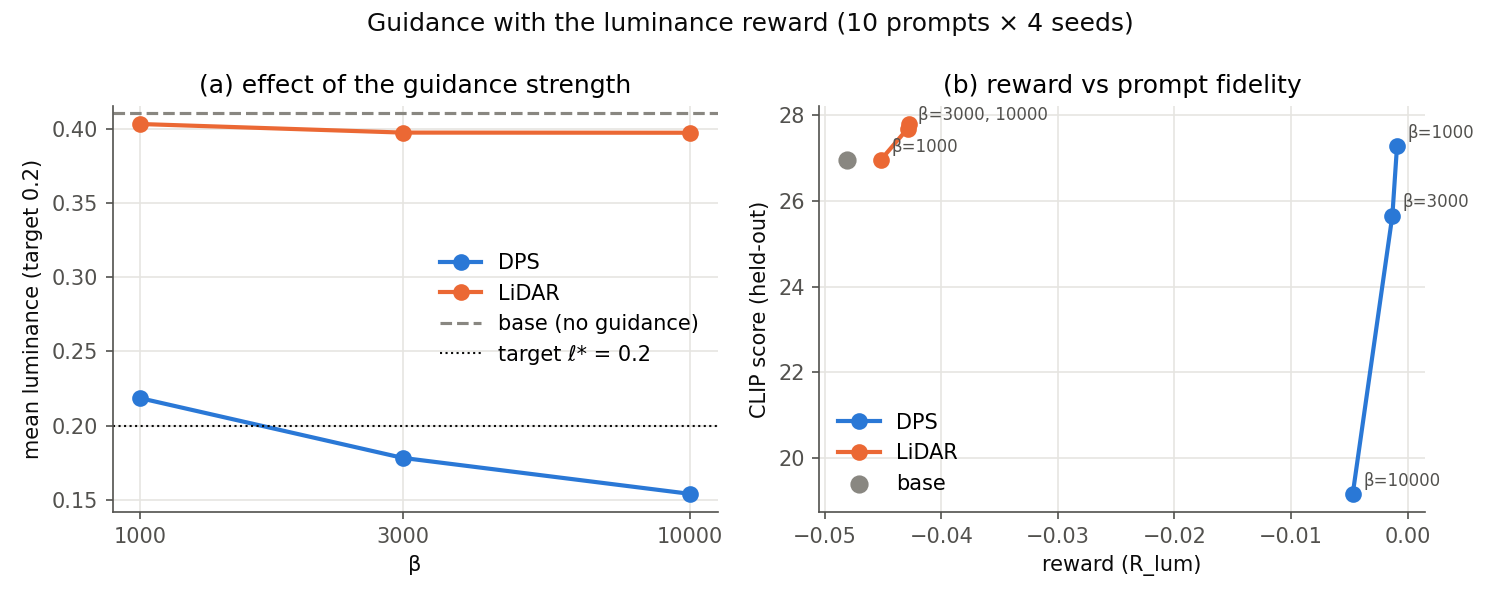
\includegraphics[width=\linewidth]{figures/luminance_curves.png}
\caption{Luminance reward. (a) Mean luminance against $\beta$: DPS crosses the target and overshoots it, LiDAR stays at the base level. (b) Reward against held-out CLIP score: DPS at $\beta=10^3$ reaches the best reward at no cost in prompt fidelity, then CLIP collapses.}
\label{fig:lum_curves}
\end{figure}

\begin{figure}[t]
\centering
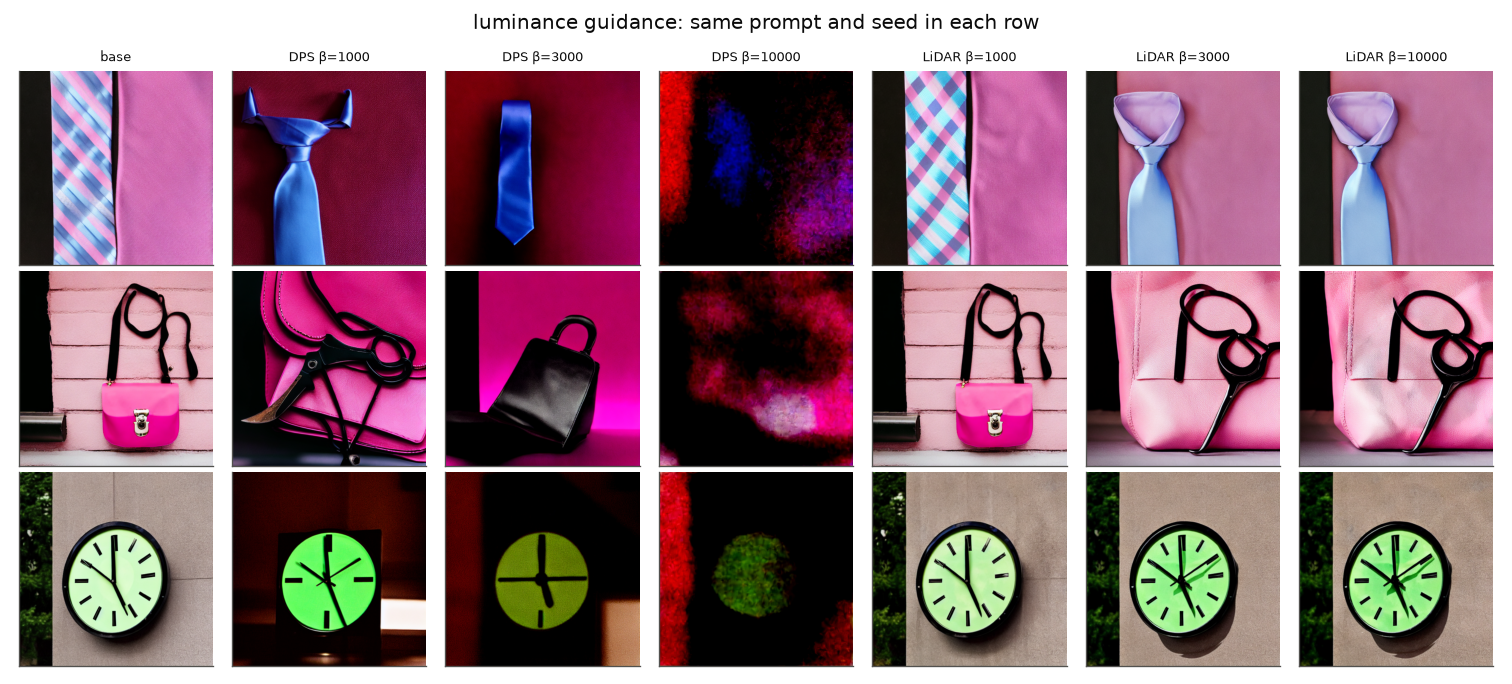
\includegraphics[width=\linewidth]{figures/luminance_grid.png}
\caption{Luminance reward, same prompt and seed in each row. DPS at $\beta=10^3$ produces naturally dark compositions that keep the prompt content; at $\beta=10^4$ the images degenerate. LiDAR changes the composition at $\beta\geq3\cdot10^3$ without darkening the image, and gives identical images at $3\cdot10^3$ and $10^4$.}
\label{fig:lum_grid}
\end{figure}

Table~\ref{tab:lum} and Figures~\ref{fig:lum_curves}--\ref{fig:lum_grid} support \ref{h:eff}. At $\beta=10^3$, DPS brings the mean luminance from $0.411$ to $0.219$ and the reward from $-0.048$ to $-0.0009$, with a CLIP score unchanged from the base ($27.28$ vs.\ $26.96$). The guided images are not darkened copies of the base images: their composition changes (dark backgrounds, studio lighting) while the objects of the prompt remain (Figure~\ref{fig:lum_grid}). This is consistent with the factor $\sigma_t$ in~\eqref{eq:guided}, close to $1$ in the first steps, where the global layout is decided. LiDAR moves the mean luminance only from $0.411$ to $0.398$.

The results also support \ref{h:bias}: beyond $\beta=10^3$, DPS overshoots the target ($0.178$, then $0.154$) and its reward \emph{decreases} with $\beta$, from $-0.0009$ to $-0.0047$. At $\beta=10^4$ the images lose all content (Figure~\ref{fig:lum_grid}), and both the held-out CLIP score ($19.16$) and ImageReward ($-2.09$) drop sharply, as predicted by \ref{h:hack}.

\subsection{ImageReward}

\begin{table}[t]
\centering
\caption{ImageReward. Means over 10 prompts $\times$ 4 seeds. Bold: best guided reward.}
\label{tab:ir}
\small
\begin{tabular}{llcccccc}
\toprule
Method & $\beta$ & ImageReward$\uparrow$ & CLIP$\uparrow$ & mean lum. & dist. & time (s/img) \\
\midrule
Base & -- & $-0.87$ & 26.96 & 0.411 & 0 & 0.47 \\
\midrule
\multirow{3}{*}{DPS} & 3 & $-0.63$ & 27.05 & 0.415 & 0.10 & 3.76 \\
 & 10 & $-0.16$ & 27.15 & 0.421 & 0.18 & 3.75 \\
 & 30 & $\bm{+0.31}$ & 26.36 & 0.422 & 0.23 & 3.76 \\
\midrule
\multirow{3}{*}{LiDAR} & 3 & $-0.98$ & 26.50 & 0.409 & 0.06 & 0.90 \\
 & 10 & $-0.90$ & 26.88 & 0.409 & 0.07 & 0.90 \\
 & 30 & $-0.97$ & 27.09 & 0.409 & 0.10 & 0.91 \\
\bottomrule
\end{tabular}
\end{table}

\begin{figure}[t]
\centering
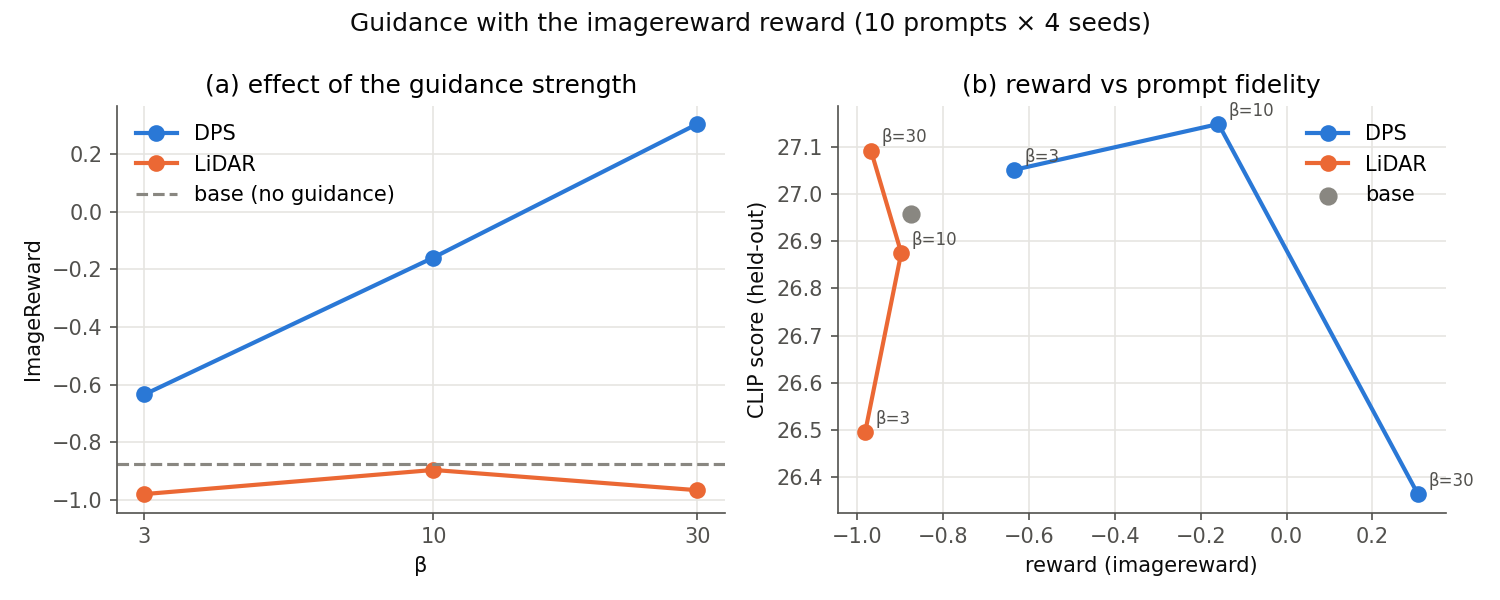
\includegraphics[width=\linewidth]{figures/imagereward_curves.png}
\caption{ImageReward. (a) DPS increases the reward steadily with $\beta$; LiDAR does not improve it. (b) CLIP is stable for DPS up to $\beta=10$ and decreases at $\beta=30$.}
\label{fig:ir_curves}
\end{figure}

\begin{figure}[t]
\centering
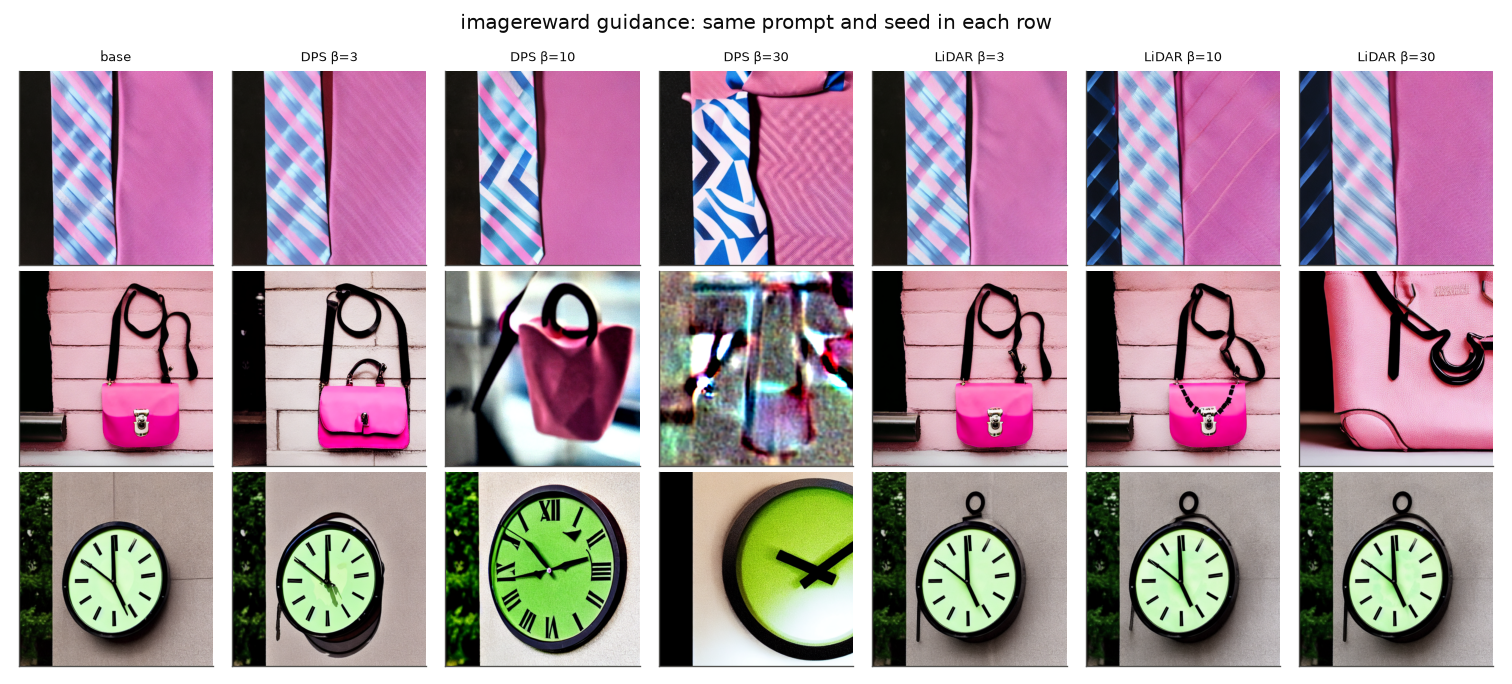
\includegraphics[width=\linewidth]{figures/imagereward_grid.png}
\caption{ImageReward, same prompt and seed in each row. At $\beta=10$, DPS increases contrast and stylisation but loses the scissors of the second prompt; at $\beta=30$ the second image becomes a noise-like texture that ImageReward nevertheless scores highly.}
\label{fig:ir_grid}
\end{figure}

On the learned reward (Table~\ref{tab:ir}, Figures~\ref{fig:ir_curves}--\ref{fig:ir_grid}), DPS raises ImageReward monotonically from $-0.87$ to $+0.31$, i.e.\ by more than one standard deviation of the standardised score, with a stable CLIP score up to $\beta=10$. LiDAR does not improve the reward at any $\beta$; its deviations from the base are within noise. Part of the gain of DPS is, however, illusory (\ref{h:hack}): at $\beta=30$, one of the three displayed samples turns into a high-frequency, noise-like texture with no recognisable object, yet contributes to the reward increase (Figure~\ref{fig:ir_grid}). The held-out CLIP score decreases only mildly ($27.15\to26.36$), so visual inspection was necessary to detect this failure.

\subsection{Why LiDAR has almost no effect}

\begin{table}[t]
\centering
\caption{LiDAR diagnostics along one trajectory (luminance, $\beta=10^4$, first prompt, $n=16$). $\ESS$: effective sample size of the kernel weights; correction: $\sigma_t\|\nabla\log\hat h_t\|$; $\|\eps\|$ given for scale.}
\label{tab:ess}
\small
\begin{tabular}{lcccccccccc}
\toprule
$t$ & 981 & 881 & 781 & 681 & 581 & 481 & 381 & 281 & 181 & 81 \\
\midrule
$\ESS$ (out of 16) & 1.51 & 1.00 & 1.01 & 1.06 & 1.00 & 1.00 & 1.00 & 1.00 & 1.00 & 1.00 \\
correction & 8.55 & 0.01 & 0.08 & 0.84 & 0.00 & 0.00 & 0.00 & 0.00 & 0.00 & 0.00 \\
$\|\eps\|$ & 128 & 128 & 128 & 128 & 127 & 125 & 123 & 120 & 116 & 108 \\
\bottomrule
\end{tabular}
\end{table}

Table~\ref{tab:ess} confirms \ref{h:collapse}. The effective sample size is $1.5$ at the first step and $1.0$ afterwards: a single lookahead sample carries all the weight. By~\eqref{eq:lidar_grad}, a one-hot weight vector gives $w^R=w$ and a guidance term exactly equal to zero; the measured correction is about $7\%$ of $\|\eps\|$ at the first step and zero for most of the remaining ones. LiDAR therefore applies a single push at the beginning of sampling, after which the sampler follows its unguided dynamics. This accounts for all observations of Table~\ref{tab:lum}: the composition changes (pixel distance $0.11$) but the reward barely improves, and increasing $\beta$ from $3\cdot10^3$ to $10^4$ leaves the images identical because $w^R$ is already concentrated on the same sample. A second limitation is coverage: the $16$ lookahead rewards ranged from $-0.116$ to $-0.045$, i.e.\ luminances between $0.41$ and $0.54$, so no lookahead sample was close to the target and even perfect weights could only pull towards images of luminance $\approx0.41$.

\subsection{Cost}
Unguided sampling takes $0.47$\,s per image, LiDAR $0.9$\,s ($\approx2\times$, dominated by the $16\times10$ lookahead denoising steps per prompt), and DPS $3.2$--$3.8$\,s ($\approx7$--$8\times$), since each of its $50$ steps requires a decoder pass and a backward pass through reward, decoder and U-Net.

\section{Discussion}
\label{sec:discussion}

\paragraph{Does DPS sample $\pi$?}
The luminance reward depends on a single scalar, which allows a direct check. The tilt $e^{-\beta(\bar\ell-\ell^\star)^2}$ is a Gaussian bump in $\bar\ell$ of width $1/\sqrt{2\beta}$: $0.022$, $0.013$ and $0.007$ for our three values of $\beta$. Since the base luminances spread over roughly $0.3$--$0.55$, the tilt dominates and $\pi$ concentrates its mean luminance within about one width of $0.2$, slightly above it because $p$ puts more mass on brighter images. DPS is consistent with this at $\beta=10^3$ ($0.219$), but lies about $2$ and $6$ widths below the target at $3\cdot10^3$ and $10^4$. Together with the non-monotone reward, this shows that the bias of DPS grows with $\beta$, as anticipated in Section~\ref{sec:dps}. We see two plausible, non-exclusive causes, which our experiments do not separate. (i) The \emph{point-mass approximation}: early corrections are computed on the reward of a blurry posterior mean, a poor predictor of the final reward. (ii) \emph{Discretisation}: each step applies a correction proportional to $\beta$ without accounting for later corrections, so for large $\beta$ the guided dynamics become stiff and $50$ explicit steps overshoot, much like gradient descent with too large a step; once past the target, later corrections are scaled by a small $\sigma_t$ and act on an already fixed layout, which prevents recovery. Explanation (ii) predicts less overshoot with more sampling steps; (i) does not.

\paragraph{Why do the LiDAR weights collapse?}
The softmax in~\eqref{eq:lidar_w} is invariant to a common shift of the $\ell_i$; only the \emph{differences} between squared distances matter. Each squared distance is a sum of $D$ coordinate-wise terms: its common part grows like $D$ and cancels, while its sample-to-sample fluctuations grow like $\sqrt{D}$ and do not. With $2\sigma_t^2\leq2$ fixed, the log-weight gaps therefore grow with $\sqrt{D}$, and at $D=16\,384$ the closest lookahead sample dominates. This is the mechanism behind the collapse of importance weights in high-dimensional particle filters \citep{bengtsson2008curse, snyder2008obstacles}, where avoiding collapse requires a sample size exponential in the effective dimension. It implies that increasing $n$ alone cannot restore LiDAR's signal, whereas computing the weights in a lower-dimensional representation, or tempering the kernel, could.

\paragraph{Two forms of reward hacking.}
With luminance, the reward cannot be fooled: a high-reward image \emph{is} dark. Large $\beta$ instead pushes the latent off the manifold where the decoder produces natural images. ImageReward, being a neural network trained on natural images, has no meaningful output elsewhere, and its gradient contains adversarial directions: perturbations distributed over many pixels, each small, that add up to a large change of the score \citep{goodfellow2015adversarial}. This is an instance of reward over-optimisation \citep{gao2023overoptimization}. Notably, the exact target would not produce these samples: $\pi\propto p\,e^{\beta R}$ only reweights images that $p$ can produce, and adversarial textures have negligible probability under $p$. Hacking is therefore a symptom of the bias of the gradient estimator rather than of the objective~\eqref{eq:target}.

\paragraph{Gradients versus lookahead.}
The reward gradient provides a direction at every step and everywhere in latent space, including towards regions that $p$ rarely visits; LiDAR only knows $n$ points and, in high dimension, effectively one. The price of the gradient is a $\approx4\times$ higher cost than LiDAR, the need for a differentiable reward, and a bias that requires a moderate $\beta$ and a held-out metric.

\section{Limitations}
\label{sec:limitations}
\begin{itemize}[leftmargin=*, itemsep=2pt]
  \item \textbf{Scale.} $10$ prompts and $4$ seeds per configuration, mostly of the GenEval ``two coloured objects'' type, and no confidence intervals; differences in CLIP score below about one point should not be considered significant.
  \item \textbf{No exact sampling of $\pi$.} We characterise the bias of DPS but do not correct it, and we do not separate its two candidate causes.
  \item \textbf{Compute matching.} LiDAR was run with $n=16$ and is about four times cheaper than DPS. We did not run a compute-matched comparison ($n\approx100$); the collapse analysis predicts a small gain, which remains to be verified. The original LiDAR paper may use settings that mitigate the collapse.
  \item \textbf{Metrics.} A single held-out metric (CLIP); HPSv2 \citep{wu2023hpsv2} was not used. The pixel distance to the base image is only a proxy for the divergence from $p$.
  \item \textbf{Rewards.} Two rewards; spatial and symmetry rewards were not studied.
\end{itemize}

\section{Conclusion and future work}
\label{sec:conclusion}
When the reward is differentiable, differentiating the Tweedie approximation of the expected future reward is a simple and much more effective guidance signal than lookahead samples in the latent space of Stable Diffusion, at a moderate inverse temperature. It is, however, a biased estimator whose error grows with $\beta$ and manifests as target overshoot and reward hacking, while LiDAR fails for a structural reason, the collapse of its kernel weights in high dimension, that additional samples alone are unlikely to fix.

Three directions follow. (i) \emph{Correcting the bias}: use the gradient-guided transition as the proposal of a sequential Monte Carlo sampler with a stochastic sampler ($\eta>0$) and importance weights $\hat h_s(x_s)\,p(x_s\mid x_t)/\big(\hat h_t(x_t)\,q(x_s\mid x_t)\big)$, in the spirit of the twisted diffusion sampler \citep{wu2023tds}, which keeps the efficiency of the gradient and targets $\pi$ as the number of particles grows; weight degeneracy in high dimension must then be monitored as well. (ii) \emph{Separating the causes of overshoot} by varying the number of sampling steps and replacing the point mass by a Monte Carlo average of $e^{\beta R}$ over a Gaussian approximation of the posterior. (iii) \emph{Restoring lookahead guidance in high dimension} by computing kernel weights in a downsampled latent space or with a tempered kernel.

\section*{Reproducibility}
The code (sampler, rewards, both estimators, generation, evaluation and figure scripts) is available at \url{https://github.com/yassine11102003/test_time_guidance}. Each table and figure is produced by one command listed in the repository README. All experiments ran on a single NVIDIA H100 (80\,GB).

\bibliographystyle{plainnat}
\bibliography{references}

\end{document}
